\documentclass{beamer} 
\usetheme{Boadilla}
\usecolortheme{albatross}
\setbeamercovered{transparent}
%\usetheme{default} 
%\useoutertheme{umbcfootline} 
%\setbeamertemplate{background canvas}[vertical shading][bottom=red!20,top=yellow!30] 
\usepackage{hyperref}\usepackage[utf8x]{inputenc}
\usepackage[spanish]{babel}
%\usepackage{beamerthemeshadow}
%\beamersetuncovermixins{\opaqueness<1>{25}}{\opaqueness<2->{15}}

\usepackage{lmodern}

\title{Introducción a Java}   
\author{Manuel J. Molino\and Luis Molina}
\institute{IES Virgen del Carmen\and Departamento de informatica}
\date{\today} 


% Adicional intercala package{beamerthemeshadow} 
%\usepackage{beamerthemeshadow}
%  causa que elementos que aparece en el futuro 
%  escribe ligero 
%\beamersetuncovermixins{\opaqueness<1>{25}}{\opaqueness<2->{15}}
% funciona por tablas tambien cuando aplica teTeX
\begin{document}


\begin{frame}
\titlepage %portada
\end{frame} 

\begin{frame}
\frametitle{Índice}
\tableofcontents
\end{frame} 


\section{Historia Java} 

\begin{frame}
\frametitle{Oracle Java} 
\begin{figure}

\includegraphics[scale=0.35]{imagenes/java.jpg} 
\caption{logotipo}
\end{figure} 
\end{frame}

\section{Introducción}

\begin{frame}
\frametitle{Introducción I}
\begin{small}
\begin{itemize}[<+->]
\item Es un lenguaje de programación originalmente desarrollado por James Gosling de Sun Microsystems (la cual fue adquirida por la compañía Oracle).
\item Originalmente se llamó \emph{Oak}
\item Fue diseñado para ser usado embebido en chips.
\item Cuando se rediseñó para Internet se le llamó \emph{Java}
\item El lenguaje deriva mucho de su sintaxis de C y C++.
\item Tiene menos facilidades de bajo nivel que cualquiera de ellos.
\item Las aplicaciones de Java son generalmente compiladas a bytecode (clase Java) que puede correr en cualquier máquina virtual Java (JVM) sin importar la arquitectura de la computadora.
\item Java es un lenguaje de programación de propósito general, concurrente, basado en clases, y orientado a objetos.
\item Su intención es permitir que los desarrolladores de aplicaciones escriban el programa una vez y lo ejecuten en cualquier dispositivo (conocido en inglés como WORA, o "write once, run anywhere"), lo que quiere decir que el código que es ejecutado en una plataforma no tiene que ser recompilado para correr en otra.
\end{itemize} 
\end{small}
\end{frame}



\begin{frame} 
\frametitle{Introducción II}
\begin{itemize}[<+->]
\item A partir del 2012, uno de los lenguajes de programación más populares en uso, particularmente para aplicaciones de cliente-servidor de web, con unos 10 millones de usuarios reportados.
\item La compañía Sun desarrolló la implementación de referencia original para los compiladores de Java, máquinas virtuales, y librerías de clases en 1991 y las publicó por primera vez en el 1995.
\item A partir de mayo del 2007, en cumplimiento con las especificaciones del Proceso de la Comunidad Java, Sun volvió a licenciar la mayoría de sus tecnologías de Java bajo la Licencia Pública General de GNU.
\item Otros también han desarrollado implementaciones alternas a estas tecnologías de Sun, tales como el Compilador de Java de GNU y el GNU Classpath.
\item La última versión es \href{https://en.wikipedia.org/wiki/Java_version_history}{\emph{Consultar}}. 
\end{itemize} 
\end{frame}


\section{Características} 

\begin{frame}
\frametitle{Filosofía}
\begin{itemize}[<+->]
\item Debería usar el paradigma de la programación orientada a objetos.
\item Debería permitir la ejecución de un mismo programa en múltiples sistemas operativos.
\item Debería incluir por defecto soporte para trabajo en red.
\item Debería diseñarse para ejecutar código en sistemas remotos de forma segura.(RMI o CORBA)
\item Debería ser fácil de usar y tomar lo mejor de otros lenguajes orientados a objetos, como C++.
\end{itemize} 
\end{frame}

\section{Entornos de desarrollo}
\begin{frame}
\frametitle{Dispositivos móviles y sistemas empotrados}
\begin{itemize}[<+->]
\item J2ME (Java 2 Platform, Micro Edition), una versión del entorno de ejecución Java reducido y altamente optimizado. 
\item Es posible encontrar microprocesadores diseñados para ejecutar bytecode Java y software Java para tarjetas inteligentes (JavaCard), teléfonos móviles, buscapersonas, set-top-boxes, sintonizadores de TV y otros pequeños electrodomésticos.
\item El modelo de desarrollo de estas aplicaciones es muy semejante a las \emph{applets} de los navegadores salvo que en este caso se denominan \emph{MIDlelts}
\end{itemize} 
\end{frame}

\begin{frame}
\frametitle{Navegadores web}
\begin{itemize}[<+->]
\item Uso de pequeñas aplicaciones (Applets) en Java que luego pueden ser incrustadas en una página HTML para que sean descargadas y ejecutadas por el navegador web. 
\item Estas mini-aplicaciones se ejecutan en una JVM que el navegador tiene configurada como extensión (plug-in) en un contexto de seguridad restringido configurable para impedir la ejecución local de código potencialmente malicioso.
\item La aparición posterior de otras alternativas (aplicaciones web dinámicas de servidor) dejó un reducido ámbito de uso para esta tecnología.  
\item Otras tecnologías similares pueden ser: ActiveX de Microsoft, Flash, Java Web Start, etc.
\end{itemize} 
\end{frame}

\begin{frame}
\frametitle{Servidores}
\begin{itemize}[<+->]
\item Las especificaciones de Servlets y JSP (Java Server Pages).
\item La especificación de Servlets y JSPs define un API de programación.
\item Hoy en día se usa framework como es \href{https://www.1and1.es/digitalguide/paginas-web/desarrollo-web/spring-framework-la-columna-vertebral-de-java/}{\emph{Spring}}
\end{itemize}
\end{frame}

\begin{frame}
\frametitle{Aplicaciones de escritorio}
\begin{itemize}[<+->]
\item Hoy en día existen multitud de aplicaciones gráficas de usuario basadas en Java.
\item En las primeras versiones de la plataforma Java existían importantes limitaciones en las APIs de desarrollo gráfico (AWT). 
\item Desde la aparición de la biblioteca Swing la situación mejoró substancialmente.
\item Posteriormente con la aparición de bibliotecas como SWT hacen que el desarrollo de aplicaciones de escritorio complejas y con gran dinamismo, usabilidad, etc. sea relativamente sencillo.
\end{itemize}
\end{frame}

\begin{frame}
\frametitle{Android}
\begin{itemize}[<+->]
\item Android hace uso del lenguaje de programación Java, un lenguaje que es propiedad de Oracle desde 2010 tras haber comprado a su creador original, Sun. 
\item Esto ha acarreado múltiples disputas legales entre Google y Oracle, que todavía a día de hoy no está del todo aclarado.
\item La noticia ahora es que, a partir de Android N, Google ya no usará más las APIs Java de Oracle.
\item Usará \emph{OpenJDK} la versión de código abierto del Java Development Kit.
\item Hoy en día, Google tiene la intención de usar el lenguaje \href{https://es.wikipedia.org/wiki/Kotlin\_(lenguaje\_de\_programaci\%C3\%B3n)}{\emph{kotlin}}
\end{itemize}
\end{frame}

\section{API} 

\begin{frame}
\frametitle{Application Program Interface} 
Hay tres plataformas en un intento por cubrir distintos entornos de aplicación
\pause
\begin{description}[<+->]
\item[Java ME] orientada a entornos de limitados recursos, como teléfonos móviles, PDAs,\dots
\item[Java SE] para entornos de gama media y estaciones de trabajo. Aquí se sitúa al usuario medio en un PC de escritorio.
\item[Java EE] orientada a entornos distribuidos empresariales o de Internet.
\end{description}
\pause
Las clases en las APIs de Java se organizan en grupos disjuntos llamados paquetes. Cada paquete contiene un conjunto de interfaces, clases y excepciones relacionadas. La información sobre los paquetes que ofrece cada plataforma puede encontrarse en la documentación de ésta.
\end{frame}


\section{Instalación}

\begin{frame}[fragile]
\frametitle{JRE y JDK}
\begin{itemize}[<+->]
\item \emph{JVM} es la máquina virtual de Java. Es la aplicación donde corren los programas hechos en Java, es nativa del sistema operativo 
\item El \emph{JRE} (Java Runtime Environment) es un conjunto de utilidades de Java contiene la JVM. 
\item El \emph{JDK} (Java Development Kit) es el kit para desarrolladores, contiene entre otras cosas el JRE y por tanto a la JVM.
\end{itemize}
\end{frame}

\begin{frame}
\frametitle{Diagrama conceptual de Java}
\begin{figure}
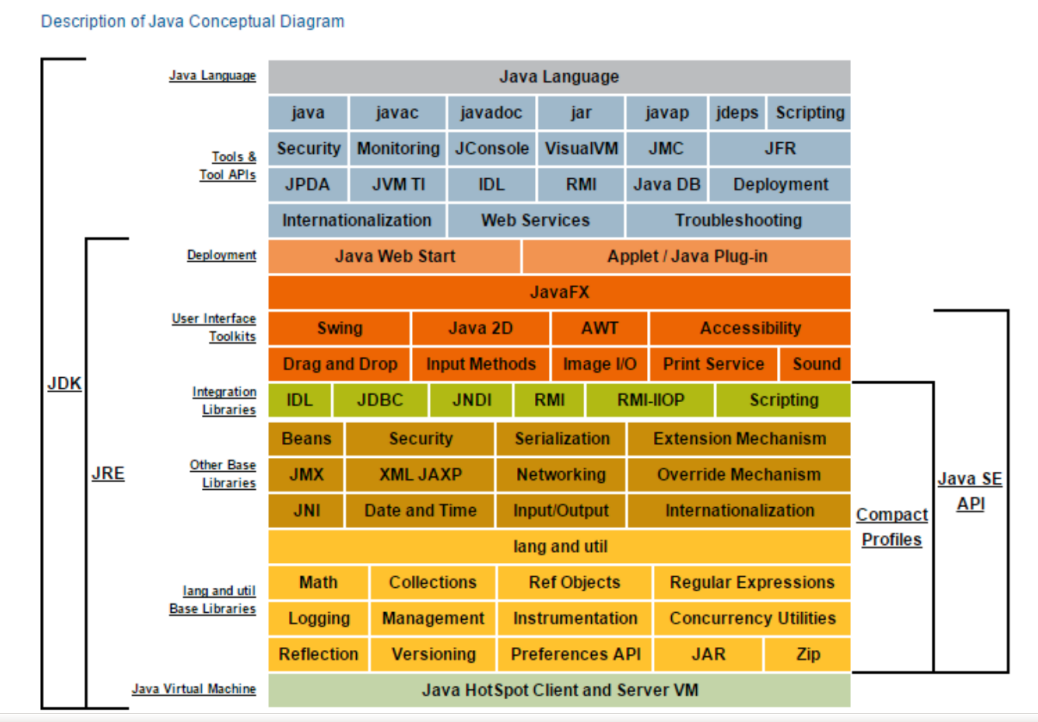
\includegraphics[scale=0.4]{imagenes/java.png}
\end{figure}
\end{frame}

\begin{frame}
\frametitle{OpenJDK}
\framesubtitle{IcedTea}
\begin{itemize}[<+->]
\item La versión libre de la plataforma de desarrollo Java.
\item Es posible de esta manera crear \emph{software libre} con Java.
\item Pero su ejecución depende de la máquina virtual Java, que no es \emph{software libre}.
\item A esto \emph{Richard Stallman} le donominó \emph{la trampa de Java}.
\item Debido a las múltiples dispusta de patentes entre \emph{Oracle} y \emph{Google}, a partir de \emph{Android N}, Google ya no usará más las \emph{APIs Java de Oracle}, en favor de \emph{OpenJDK}, la versión de código abierto del \emph{Java Development Kit}.
\end{itemize}
\end{frame}

\begin{frame}
\frametitle{Java y Oracle}
En la página oficial de oracle, encontramos para descargar los siguientes productos relacionados con Java:
\begin{itemize}[<+->]
\item Java SE.
\item Java ME.
\item Java EE.
\end{itemize}
\end{frame}


%\begin{frame}
%\frametitle{JVM} 
%El API de Java y la Máquina Virtual Java forman una capa intermedia (Java platform) que aísla el programa Java de las especificidades del hardware 
%\begin{figure}
%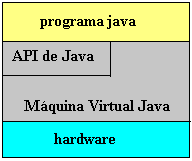
\includegraphics[scale=0.9]{imagenes/jvm1.png}
%\caption{JVM}
%\end{figure}
%\end{frame}

\begin{frame}
\frametitle{JVM}
\framesubtitle{Las tareas principales de la JVM son:}
\begin{itemize}[<+->]
\item Reservar espacio en memoria para los objetos creados.
\item Liberar la memoria no usada (garbage collection).
\item Asignar variables a registros y pilas.
\item Llamar al sistema huésped para ciertas funciones, como los accesos a los dispositivos.
\item Vigilar el cumplimiento de las normas de seguridad de las aplicaciones Java
\item Qué son:
\begin{enumerate}
\item Las referencias a arrays son verificadas en el momento de la ejecución del programa
\item No hay manera de manipular de forma directa los punteros
\item La JVM gestiona automáticamente el uso de la memoria, de modo que no queden huecos.
\item No se permiten realizar ciertas conversiones (casting) entre distintos tipos de datos.

\end{enumerate}
\end{itemize}
\end{frame}

\begin{frame}
\frametitle{Primer programa}
\framesubtitle{Requisitos}
\begin{enumerate}[<+->]
\item Un editor de texto para escribir el código:
\begin{description}
\item[GNU/Linux] podemos usar editor por defecto \emph{kwrite} para KDE o \emph{gedit} para GNOME, tambiem \emph{vim}, \emph{geany}, \emph{emacs}, \dots
\item[Windows] \emph{Notepad++}, \emph{geany}
\end{description}  
\item Tambien existen IDE de desarrollo que veremos posteriormente como \emph{eclipse}, \emph{netbeans}, \emph{JDeveloper}, \emph{IntelliJ IDEA},  \dots 
\item Compilamos el programa con el compilador, por ejemplo \emph{javac} el cual creará los correspondientes \emph{bytecodes} en un programa con extensión \emph{.class}
\item Ejecutamos el programa con \emph{java programa.class}
\end{enumerate}
\end{frame}



\begin{frame}[fragile]
\frametitle{Hola Mundo} 
El programa lo denominamos \alert{HolaMundo.java}
\begin{verbatim}
public class HolaMundo {
        public static void main(String[] args) {
                System.out.println("Hola Mundo");
        }
}
\end{verbatim} 
\pause
\begin{itemize}[<+->]
\item Compilamos con \alert{javac HolaMundo.java}
\item Ejecutamos con \alert{java HolaMundo}
\end{itemize}
\end{frame}

\begin{frame}
\frametitle{Codigo} 
\begin{figure}
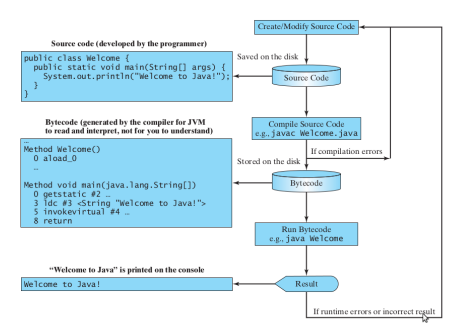
\includegraphics[scale=0.6]{imagenes/codigo.png} 
\caption{Proceso edicion, compilación y ejecución}
\end{figure} 
\end{frame}

\begin{frame}
\frametitle{jshell} 
\emph{JShell} es el primer y oficial modo REPL (Read-Eval-Print-Loop), una herramienta dela línea de comandos que nos permite ejecutar sentencias de java sin tenern que usar clases ni métodos.\\
Esta herramienta podemos usarla desde la versión 9 de java.\\
\begin{center}
\href{https://aboullaite.me/jshell-java9/}{\emph{Ejemplo de uso}}

\end{center}
\end{frame}


\begin{frame}
\frametitle{PATH y CLASSPATH}
\begin{block}{path}
Es una variable de entorno de los sistemas operativos POSIX y los sistemas de Microsoft,en ella se especifican las rutas en las cuales el intérprete de comandos debe buscar los programas a ejecutar.
\end{block}
\pause
\begin{block}{classpath}
En el lenguaje de programación Java se entiende por Classpath una opción admitida en la línea de órdenes o mediante variable de entorno que indica a la Máquina Virtual de Java dónde buscar paquetes y clases definidas por el usuario a la hora de ejecutar programas.
\end{block}
\end{frame}



\begin{frame}
\frametitle{Javadoc}
\begin{itemize}[<+->]
\item Es una utilidad de Oracle para la generación de documentación de APIs en formato HTML a partir de código fuente Java.  
\item Javadoc es el estándar de la industria para documentar clases de Java.
\item La mayoría de los IDEs los generan automáticamente.
\item Para generar APIs con Javadoc han de usarse etiquetas (tags) de HTML o ciertas palabras reservadas precedidas por el carácter ${@}$
\item Etiquetas
\begin{description}
\item[$@$author] Nombre del desarrollador.
\item[$@$param] Definición de un parámetro de un método.
\item[$@$return] Informa de lo que devuelve un método.
\item[$@$version] Versión del método o clase.
\end{description}
\end{itemize}
\end{frame}

\begin{frame}[fragile]
\frametitle{Programa hola mundo con anotaciones} 
\begin{verbatim}
//: HolaMundo.java
/** Primer programa en Java
 *  Realizamos el típico programa
 *  Hola Mundo
 * @author Manuel Molino
 * @author correo@iesvirgendelcarmen.com
 * @version 1.0
*/
public class HolaMundo {
        public static void main(String[] args) {
                System.out.println("Hola Mundo");
        }
}
\end{verbatim}
\pause
Compilamos exactemente igual que antes y generamos documentación con \alert{javadoc HolaMundo.java -author -version}
\end{frame}

\begin{frame}[fragile]
\frametitle{Automatización de tareas}
\begin{verbatim} 

/home/usuario/java
               |
               |----src   (aquí están los ficheros .java)
               |----class (aquí están los ficheros .class)
               |----doc   (aquí ponemos la documentación)
               |----jar   (fichero empaquetados)
               
\end{verbatim}
\end{frame}

\begin{frame}
\frametitle{Ant}
\begin{itemize}[<+->]
\item \alert{Apache Ant} es una herramienta usada en programación para la realización de tareas mecánicas y repetitivas
\item Desarrollado en lenguaje Java y requiere la plataforma Java, apropiado para la construcción de proyectos Java.
\item Se basa en archivos de configuración XML y clases Java.
\item El archivo XML se denomina \emph{build.xml}.
\item \emph{Ant} es un proyecto de la \emph{Apache Software Foundation}. Es software open source, y se lanza bajo la licencia \emph{Apache Software}.
\end{itemize}
\end{frame}

\begin{frame}[fragile]
\frametitle{build.xml}
\begin{verbatim} 
<?xml version="1.0"?>
<project name="Proyecto">

   <target name="compila">
      <javac srcdir="./src" destdir="./class" />
   </target>
   <target name="documenta">
      <javadoc sourcefiles="./src/HolaMundoDoc.java" 
          destdir="./doc" author="true" 
          version="true" />
   </target>

</project>
\end{verbatim}
\end{frame}

\begin{frame}[fragile]
\frametitle{maven}
\begin{itemize}[<+->]
\item Es una herramienta de software para la gestión y construcción de proyectos Java 
\item Es similar en funcionalidad a \emph{Apache Ant}
\item Maven utiliza un Project Object Model (POM) para describir el proyecto de software a construir, sus dependencias de otros módulos y componentes externos, y el orden de construcción de los elementos.
\end{itemize}
\end{frame}

\section{Applet}

\begin{frame}
\frametitle{Applet}
\begin{itemize}[<+->]
\item Es una applicación escrita en el lenguaje de programación Java. Los applets de Java pueden ejecutarse en un navegador web utilizando la Java Virtual Machine (JVM), o en el AppletViewer de Sun.
\item Poseen un esquema de seguridad que permite que los applets que se ejecutan en el equipo no tengan acceso a partes sensibles (por ej. no pueden escribir archivos), 
\item Se suele incrustar en un documento HTML, es decir en una página web. Cuando un navegador carga una página web que contiene un applet, este se descarga en el navegador web y comienza a ejecutarse. 
\item Requiere el plugin de Java, que no está disponible por defecto en todos los navegadores web.
\item Puede tener vulnerabilidades que permitan ejecutar código malicioso.
\end{itemize}
\end{frame}

\begin{frame}[fragile]
\frametitle{Ejemplo applet}
\begin{verbatim}
import javax.swing.JApplet;
import javax.swing.JLabel;
/**
 * Ejemplo sencillo de applet
 * @author Chuidiang
*/
public class Uno extends JApplet {
	/**
	 * Pone un JLabel con el texto "Applet hola mundo" en el JApplet, de
	 * forma que es lo que se visualizará en el navegador.
	 */
	public void init() {
		JLabel etiqueta = new JLabel("Applet hola mundo");
		add(etiqueta);
	}
}
\end{verbatim}
\end{frame}

\begin{frame}[fragile]
\frametitle{Applet insertado en HTML}
\begin{verbatim}
<html>
   <head>
      <title>Ejemplo de Applet</title>
   </head>
   <body>
      <applet code="Uno"
         width="500" height="200">
      Debes tener instalado java
      </applet>
   </body>
</html>
\end{verbatim}
\pause
Se puede ejecutar en un navegador o appletviewer uno.html
\end{frame}










\begin{frame}
\frametitle{Preguntas} 
\begin{figure}

\includegraphics[scale=0.9]{imagenes/dudas.png} 
\caption{Lenguaje máquina}
\end{figure} 
\end{frame}


\end{document}

